\documentclass[11pt,a4paper]{article}

\usepackage[utf8]{inputenc}
\usepackage[T1]{fontenc}
\usepackage[margin=2.5cm]{geometry}
\usepackage{amsmath}
\usepackage{booktabs}
\usepackage{graphicx}
\usepackage{float}
\usepackage{caption}
\usepackage[hidelinks]{hyperref}

\graphicspath{{figures/}}
\renewcommand{\figurename}{Figura}
\renewcommand{\tablename}{Tabla}
\renewcommand{\refname}{Referencias}
\captionsetup{font=small}
\setlength{\emergencystretch}{2em}

\title{Reporte del Laboratorio: Minería de Patrones Frecuentes y Reglas de Asociación\\
\large Análisis de los Datasets: Groceries y Adult}
\author{Oscar Alfonso\\\texttt{of\_alfonso@javeriana.edu.co}
  \and Kevin Bueno\\\texttt{bueno.kevin@javeriana.edu.co}}
\date{15 de noviembre de 2026}

\begin{document}
\maketitle

\section{Contexto de los Datos}

El dataset principal se denomina \emph{Groceries} y se distribuye con el paquete
\texttt{arules} de R \cite{arules2005}. Contiene un mes de datos reales de punto de venta de
un supermercado local \cite{groceries2006}: cada fila es un recibo (transacción) y cada columna
es un producto (ítem) que puede estar o no presente en el recibo. Para el tercer reto se
utilizó además el dataset \emph{Adult}, derivado del censo de Estados Unidos \cite{adult1996},
que \texttt{arules} entrega ya discretizado en formato transaccional.

El objetivo del laboratorio es descubrir qué productos tienden a comprarse juntos mediante
minería de conjuntos frecuentes (\emph{Eclat} \cite{zaki2000}) y reglas de asociación
(\emph{Apriori} \cite{agrawal1994}). Una regla $A \Rightarrow B$ se evalúa con tres medidas:
\begin{equation}
  \begin{gathered}
    \text{supp}(A \Rightarrow B) = P(A \cup B), \qquad
    \text{conf}(A \Rightarrow B) = \frac{\text{supp}(A \cup B)}{\text{supp}(A)}, \\[4pt]
    \text{lift}(A \Rightarrow B) = \frac{\text{supp}(A \cup B)}{\text{supp}(A)\,\text{supp}(B)}.
  \end{gathered}
  \label{eq:medidas}
\end{equation}
El soporte mide qué tan frecuente es la combinación, la confianza qué tan seguido aparece $B$
cuando aparece $A$, y el \emph{lift} cuánto más (o menos) frecuente es la combinación respecto
a lo esperado si $A$ y $B$ fueran independientes. Un \emph{lift} mayor que 1 indica correlación
positiva; menor que 1, correlación negativa.

\section{Exploración de Datos}

\subsection{Dimensiones y densidad}

La Tabla~\ref{tab:summary} resume la salida de \texttt{summary(Groceries)}. La matriz es muy
dispersa: solo el 2.6\% de las celdas está ocupado, lo que equivale a 4.4 ítems por recibo en
promedio sobre 169 posibles. La distribución del tamaño de los recibos es asimétrica: 2\,159
recibos (22\%) contienen un único ítem, la mediana es 3 y el máximo es 32.

\begin{table}[H]
  \centering
  \caption{Resumen del dataset \emph{Groceries}}
  \label{tab:summary}
  \begin{tabular}{lr}
    \toprule
    Métrica & Valor \\
    \midrule
    Transacciones (recibos) & 9\,835 \\
    Ítems (productos) & 169 \\
    Densidad de la matriz & 0.0261 \\
    Ítems por recibo: mínimo & 1 \\
    Ítems por recibo: primer cuartil & 2 \\
    Ítems por recibo: mediana & 3 \\
    Ítems por recibo: media & 4.41 \\
    Ítems por recibo: tercer cuartil & 6 \\
    Ítems por recibo: máximo & 32 \\
    \bottomrule
  \end{tabular}
\end{table}

\subsection{Primeras transacciones}

La Tabla~\ref{tab:first5} muestra los cinco primeros recibos obtenidos con
\texttt{inspect(Groceries[1:5])}. Se observa la variedad de tamaños: desde un recibo con un
solo producto hasta recibos con cuatro.

\begin{table}[H]
  \centering
  \caption{Primeras cinco transacciones del dataset}
  \label{tab:first5}
  \begin{tabular}{cl}
    \toprule
    Recibo & Ítems \\
    \midrule
    1 & citrus fruit, semi-finished bread, margarine, ready soups \\
    2 & tropical fruit, yogurt, coffee \\
    3 & whole milk \\
    4 & pip fruit, yogurt, cream cheese, meat spreads \\
    5 & other vegetables, whole milk, condensed milk, long life bakery product \\
    \bottomrule
  \end{tabular}
\end{table}

\subsection{Frecuencia de los ítems}

El soporte de un ítem individual es la proporción de recibos que lo contienen. Para los tres
primeros ítems de la matriz, \texttt{itemFrequency(Groceries[, 1:3])} devuelve 0.0590
(\texttt{frankfurter}), 0.0940 (\texttt{sausage}) y 0.0051 (\texttt{liver loaf}).

La Figura~\ref{fig:itemfreq} presenta los 15 ítems más comprados. \texttt{whole milk} aparece
en el 25.6\% de los recibos, seguido de \texttt{other vegetables} (19.3\%), \texttt{rolls/buns}
(18.4\%), \texttt{soda} (17.4\%) y \texttt{yogurt} (14.0\%). Esta concentración tiene una
consecuencia directa sobre el análisis posterior: los ítems muy populares aparecen en el lado
derecho de muchas reglas simplemente por su frecuencia, y por eso el \emph{lift} resulta
indispensable para distinguir asociación real de popularidad.

\begin{figure}[H]
  \centering
  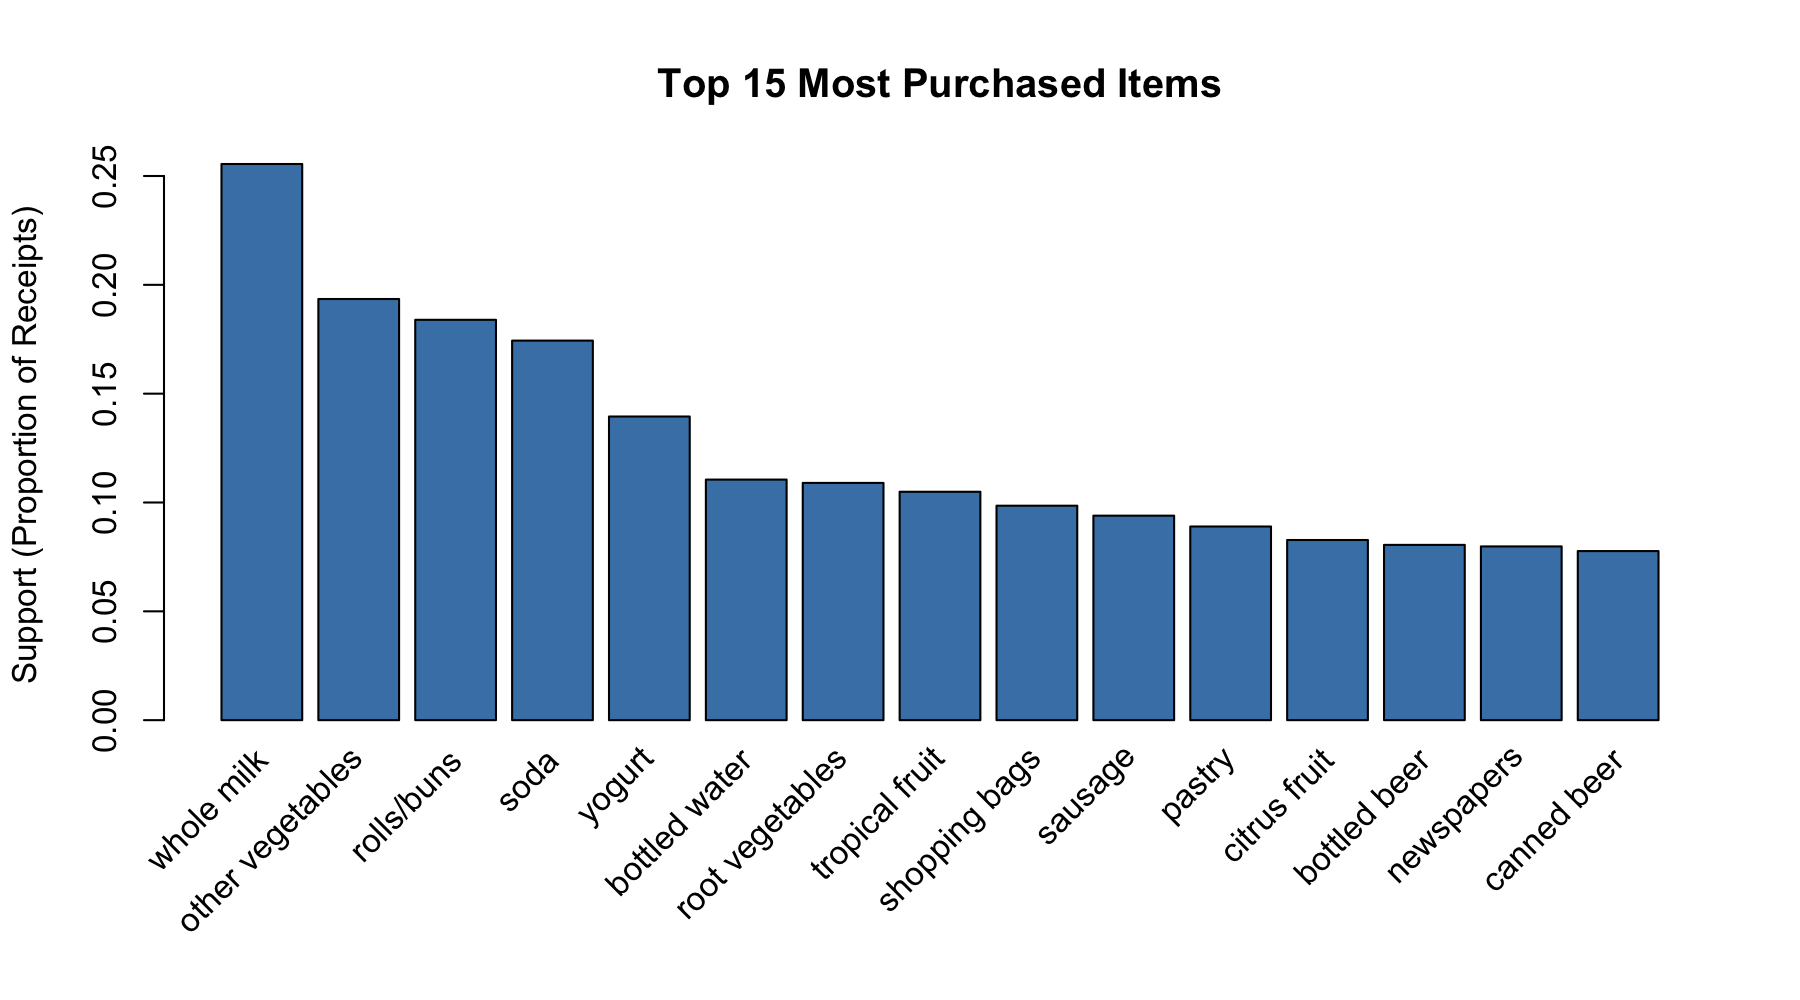
\includegraphics[width=\textwidth]{item_frequency.png}
  \caption{Los 15 ítems más comprados, medidos por soporte (proporción de recibos).}
  \label{fig:itemfreq}
\end{figure}

\section{Metodología y Análisis de Resultados}

\subsection{Conjuntos frecuentes con Eclat}

Se extrajeron los conjuntos frecuentes de al menos dos ítems con soporte mínimo de 0.01
(\texttt{supp = 0.01}, \texttt{minlen = 2}, \texttt{maxlen = 5}). El algoritmo encontró 245
conjuntos: 213 pares y 32 tríos; ningún conjunto de cuatro o más ítems alcanza el 1\% de
soporte. La Tabla~\ref{tab:eclat} lista los diez de mayor soporte.

\begin{table}[H]
  \centering
  \caption{Los 10 conjuntos frecuentes de mayor soporte (Eclat)}
  \label{tab:eclat}
  \begin{tabular}{clrr}
    \toprule
    \# & Conjunto & Soporte & Conteo \\
    \midrule
    1 & \{other vegetables, whole milk\} & 0.0748 & 736 \\
    2 & \{whole milk, rolls/buns\} & 0.0566 & 557 \\
    3 & \{whole milk, yogurt\} & 0.0560 & 551 \\
    4 & \{root vegetables, whole milk\} & 0.0489 & 481 \\
    5 & \{root vegetables, other vegetables\} & 0.0474 & 466 \\
    6 & \{other vegetables, yogurt\} & 0.0434 & 427 \\
    7 & \{other vegetables, rolls/buns\} & 0.0426 & 419 \\
    8 & \{tropical fruit, whole milk\} & 0.0423 & 416 \\
    9 & \{whole milk, soda\} & 0.0401 & 394 \\
    10 & \{rolls/buns, soda\} & 0.0383 & 377 \\
    \bottomrule
  \end{tabular}
\end{table}

Seis de los diez conjuntos contienen \texttt{whole milk} y los diez están formados
exclusivamente por ítems del top 8 de la Figura~\ref{fig:itemfreq}. Ordenar por soporte
describe, entonces, qué es popular, pero no necesariamente qué está asociado.

\subsection{Reglas de asociación con Apriori}

Se minaron reglas con \texttt{supp = 0.005}, \texttt{conf = 0.50} y \texttt{minlen = 2}, y se
obtuvieron 120 reglas. Las Tablas~\ref{tab:conf} y~\ref{tab:lift} muestran las cinco mejores
según confianza y según \emph{lift}.

\begin{table}[H]
  \centering
  \caption{Las 5 reglas de mayor confianza}
  \label{tab:conf}
  \small
  \begin{tabular}{llrrr}
    \toprule
    LHS & RHS & Soporte & Confianza & Lift \\
    \midrule
    \{tropical fruit, root vegetables, yogurt\} & whole milk & 0.0057 & 0.700 & 2.74 \\
    \{pip fruit, root vegetables, other vegetables\} & whole milk & 0.0055 & 0.675 & 2.64 \\
    \{butter, whipped/sour cream\} & whole milk & 0.0067 & 0.660 & 2.58 \\
    \{pip fruit, whipped/sour cream\} & whole milk & 0.0060 & 0.648 & 2.54 \\
    \{butter, yogurt\} & whole milk & 0.0094 & 0.639 & 2.50 \\
    \bottomrule
  \end{tabular}
\end{table}

\begin{table}[H]
  \centering
  \caption{Las 5 reglas de mayor \emph{lift}}
  \label{tab:lift}
  \small
  \begin{tabular}{llrrr}
    \toprule
    LHS & RHS & Soporte & Confianza & Lift \\
    \midrule
    \{tropical fruit, curd\} & yogurt & 0.0053 & 0.515 & 3.69 \\
    \{citrus fruit, root vegetables, whole milk\} & other vegetables & 0.0058 & 0.633 & 3.27 \\
    \{pip fruit, root vegetables, whole milk\} & other vegetables & 0.0055 & 0.614 & 3.17 \\
    \{pip fruit, whipped/sour cream\} & other vegetables & 0.0056 & 0.604 & 3.12 \\
    \{root vegetables, onions\} & other vegetables & 0.0057 & 0.602 & 3.11 \\
    \bottomrule
  \end{tabular}
\end{table}

Las dos tablas cuentan historias distintas. Las cinco reglas de mayor confianza predicen
\texttt{whole milk}: como este ítem ya está en el 25.6\% de los recibos, alcanzar una
confianza alta es comparativamente fácil y el \emph{lift} resultante es moderado (2.5 a 2.7).
Al ordenar por \emph{lift}, la primera regla es \{tropical fruit, curd\} $\Rightarrow$ yogurt:
su confianza es menor (51.5\%), pero \texttt{yogurt} solo aparece en el 14.0\% de los recibos,
de modo que quien compra fruta tropical y cuajada tiene 3.7 veces más probabilidad de llevar
yogur que un cliente promedio.

\subsection{Poda de reglas redundantes}

Una regla es redundante cuando existe otra más general (con un subconjunto de su LHS y el
mismo RHS) con confianza igual o mayor; es decir, cuando agregar ítems al antecedente no
mejora la predicción. La función \texttt{is.redundant()} eliminó una sola regla, dejando 119.
De ellas, 83 predicen \texttt{whole milk}, 35 predicen \texttt{other vegetables} y 1 predice
\texttt{yogurt}: con una confianza mínima del 50\% solo los ítems más frecuentes logran
aparecer en el consecuente.

\subsection{Preguntas dirigidas}

\textbf{¿Qué lleva a los clientes a comprar \emph{berries}?} Se minaron reglas con umbrales
más bajos (\texttt{supp = 0.002}, \texttt{conf = 0.20}) y se filtraron aquellas con
\texttt{berries} en el RHS y \emph{lift} superior a 2. El resultado es un conjunto vacío:
aunque se generan 5\,112 reglas, ninguna tiene \texttt{berries} en el consecuente.
\texttt{berries} aparece solo en el 3.3\% de los recibos y ninguna combinación de productos
eleva esa probabilidad hasta el 20\% exigido. Como verificación adicional, fuera de los
parámetros del laboratorio, se repitió la búsqueda con \texttt{conf = 0.05}: aparecen 25
reglas con \emph{lift} superior a 2 y la más fuerte es \{yogurt, whipped/sour cream\}
$\Rightarrow$ berries (confianza 14.2\%, \emph{lift} 4.28). La asociación entre
\texttt{berries} y \texttt{whipped/sour cream} existe, pero el umbral de confianza la ocultaba.

\textbf{Si alguien lleva \emph{root vegetables}, ¿qué más compra?} Entre las reglas limpias,
47 contienen \texttt{root vegetables} en el LHS. Las cinco de mayor \emph{lift}
(Tabla~\ref{tab:veggie}) predicen todas \texttt{other vegetables}, y el antecedente siempre
combina las raíces con fruta o con otro producto fresco.

\begin{table}[H]
  \centering
  \caption{Las 5 reglas de mayor \emph{lift} con \texttt{root vegetables} en el LHS}
  \label{tab:veggie}
  \small
  \begin{tabular}{llrrr}
    \toprule
    LHS & RHS & Soporte & Confianza & Lift \\
    \midrule
    \{citrus fruit, root vegetables, whole milk\} & other vegetables & 0.0058 & 0.633 & 3.27 \\
    \{pip fruit, root vegetables, whole milk\} & other vegetables & 0.0055 & 0.614 & 3.17 \\
    \{root vegetables, onions\} & other vegetables & 0.0057 & 0.602 & 3.11 \\
    \{citrus fruit, root vegetables\} & other vegetables & 0.0104 & 0.586 & 3.03 \\
    \{tropical fruit, root vegetables, whole milk\} & other vegetables & 0.0070 & 0.585 & 3.02 \\
    \bottomrule
  \end{tabular}
\end{table}

\subsection{Visualización de las reglas}

La Figura~\ref{fig:scatter} ubica las 119 reglas limpias según soporte y confianza, con el
\emph{lift} como color. La mayoría se concentra junto al umbral de soporte (0.005), y existe
un compromiso visible: las reglas de mayor confianza tienen soporte bajo, mientras que la
regla de mayor soporte (0.022) apenas supera el 50\% de confianza y tiene \emph{lift} cercano
a 2. Las reglas de \emph{lift} alto (rojo intenso) no coinciden con las de mayor confianza.

\begin{figure}[H]
  \centering
  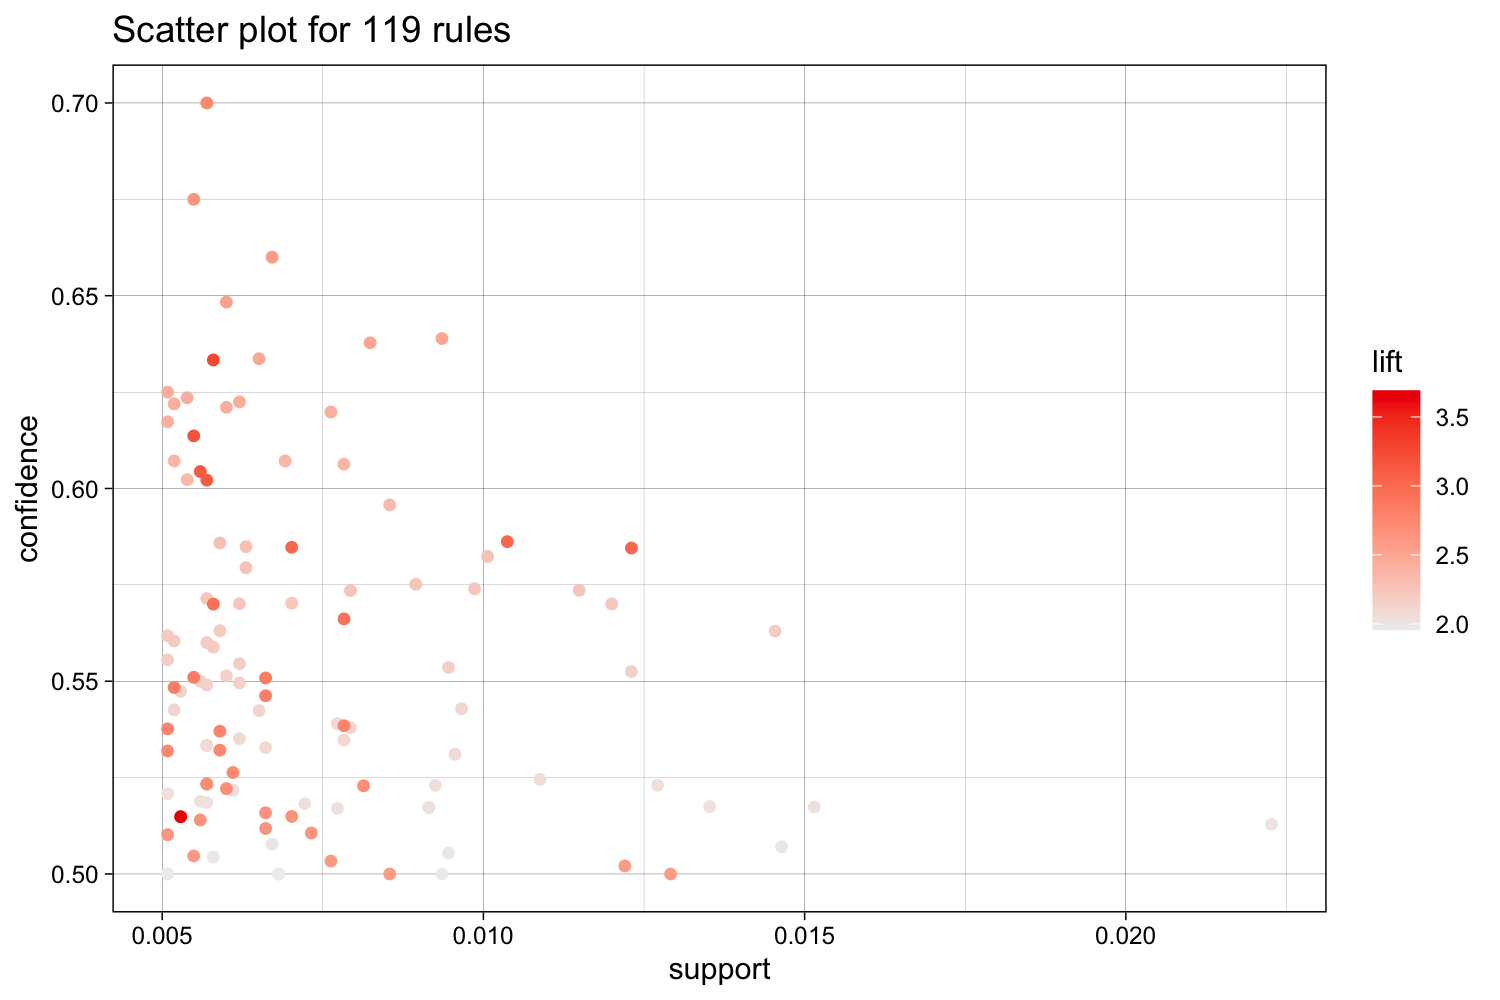
\includegraphics[width=0.85\textwidth]{scatter_rules.png}
  \caption{Soporte frente a confianza de las 119 reglas limpias; el color indica el \emph{lift}.}
  \label{fig:scatter}
\end{figure}

La Figura~\ref{fig:graph} representa las 15 reglas de mayor \emph{lift} como un grafo
dirigido. Las etiquetas son ítems y los círculos son reglas: las flechas entran al círculo
desde los ítems del LHS y salen hacia el RHS. \texttt{other vegetables} es el nodo central,
destino de 14 de las 15 reglas, y \texttt{root vegetables}, \texttt{tropical fruit} y
\texttt{whipped/sour cream} son los antecedentes más recurrentes. La única regla aislada,
\{tropical fruit, curd\} $\Rightarrow$ yogurt, es también la de mayor \emph{lift} (punto rojo
a la derecha).

\begin{figure}[H]
  \centering
  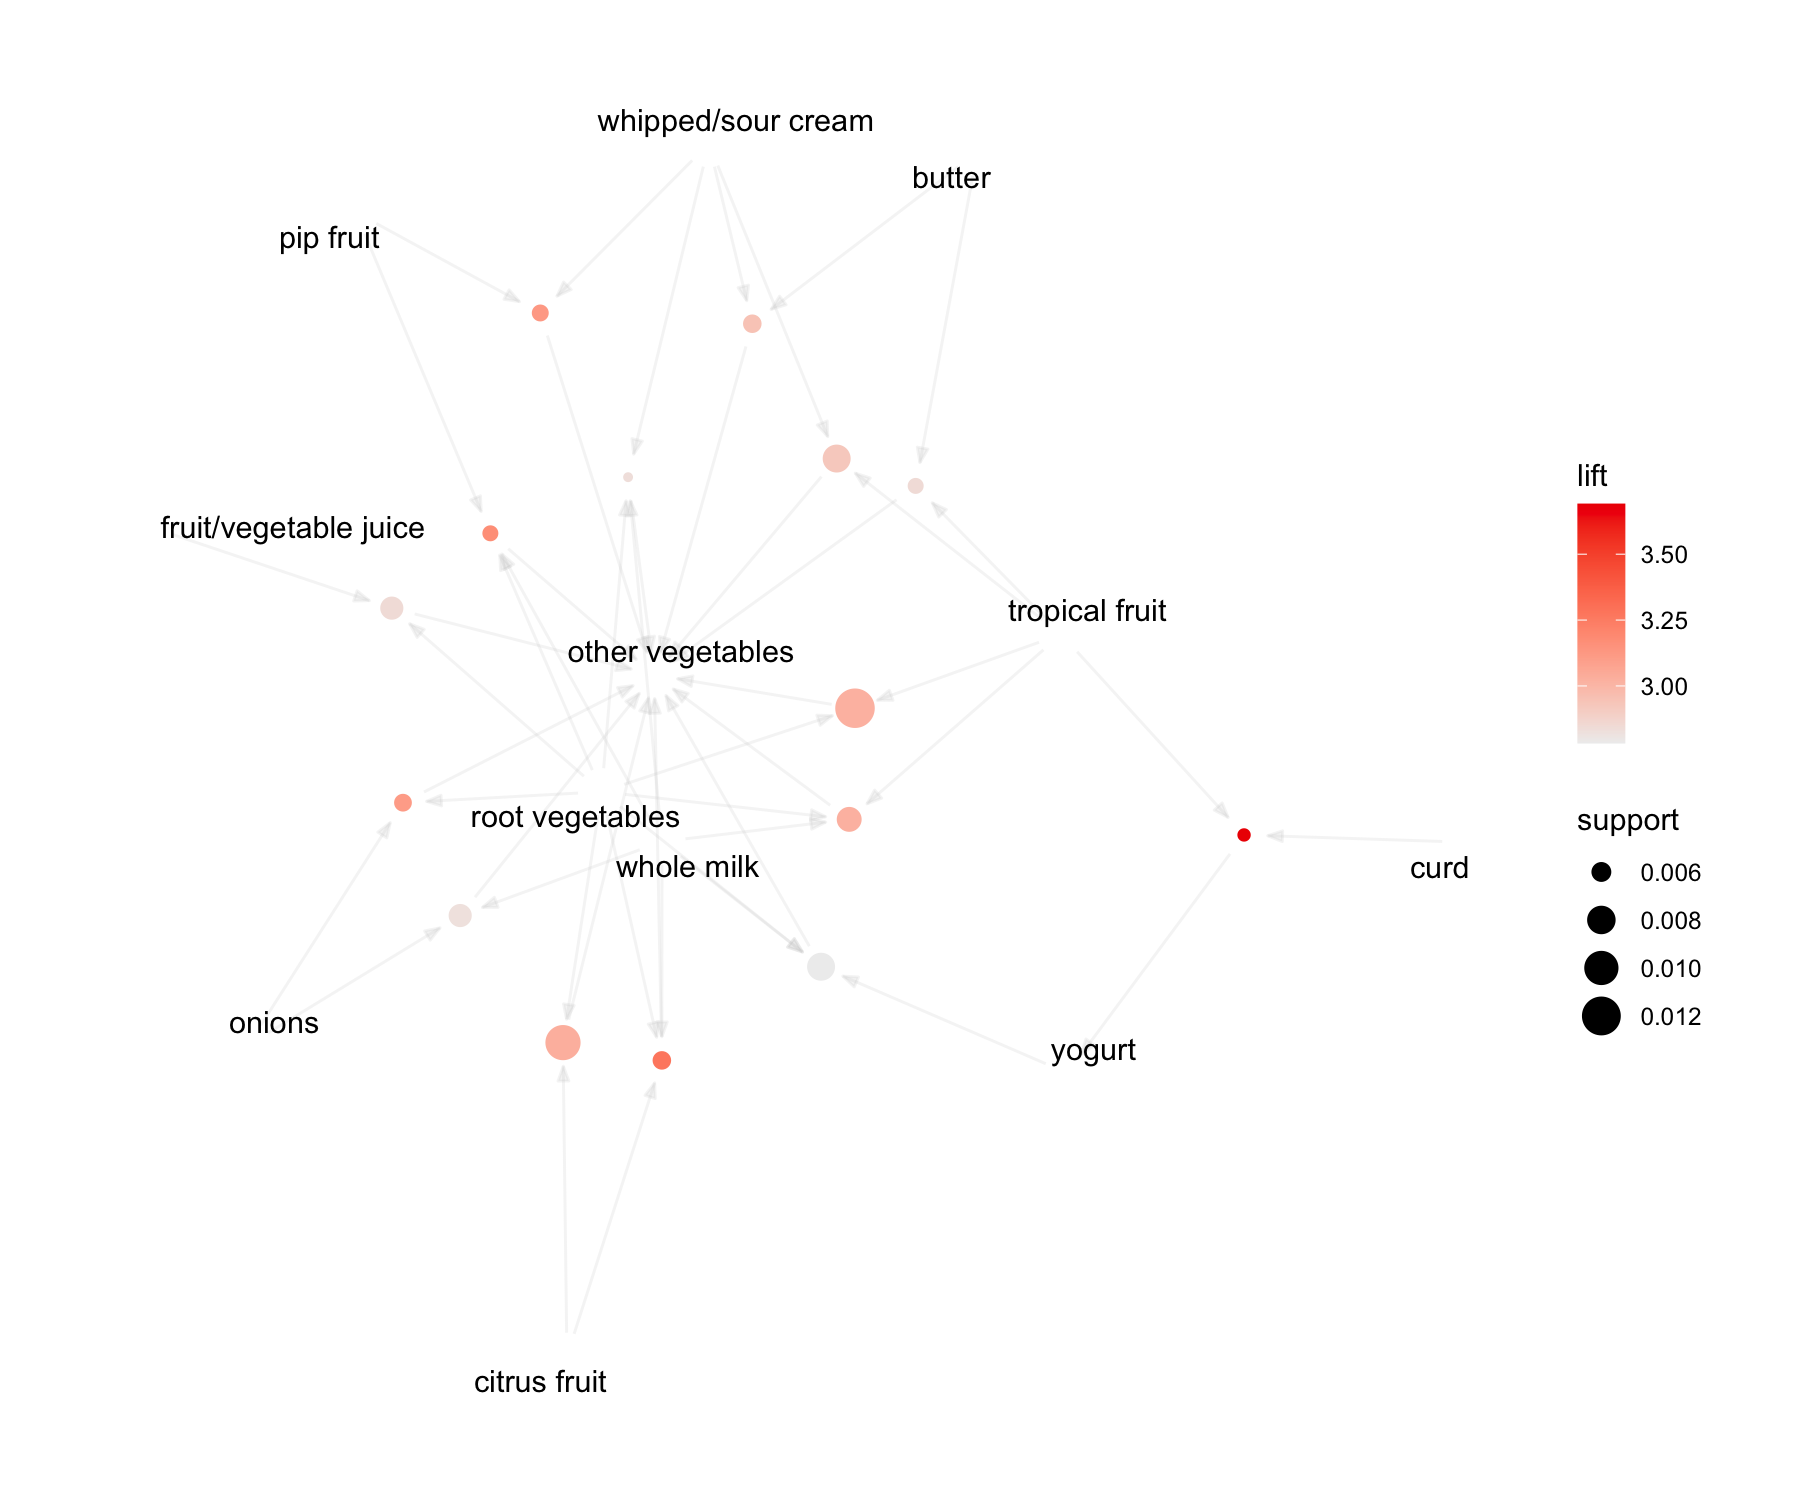
\includegraphics[width=0.9\textwidth]{graph_top15.png}
  \caption{Grafo de las 15 reglas de mayor \emph{lift}. El tamaño del círculo indica el
  soporte y el color el \emph{lift}.}
  \label{fig:graph}
\end{figure}

La Figura~\ref{fig:grouped} agrupa los antecedentes similares en columnas y muestra los tres
consecuentes en filas. Los grupos de la izquierda, formados por frutas, verduras y lácteos
frescos, concentran los \emph{lift} más altos y apuntan a \texttt{other vegetables}; los
grupos de la derecha, con productos más heterogéneos (\texttt{sausage}, \texttt{oil},
\texttt{bottled beer}), apuntan solo a \texttt{whole milk} con \emph{lift} cercano a 2.

\begin{figure}[H]
  \centering
  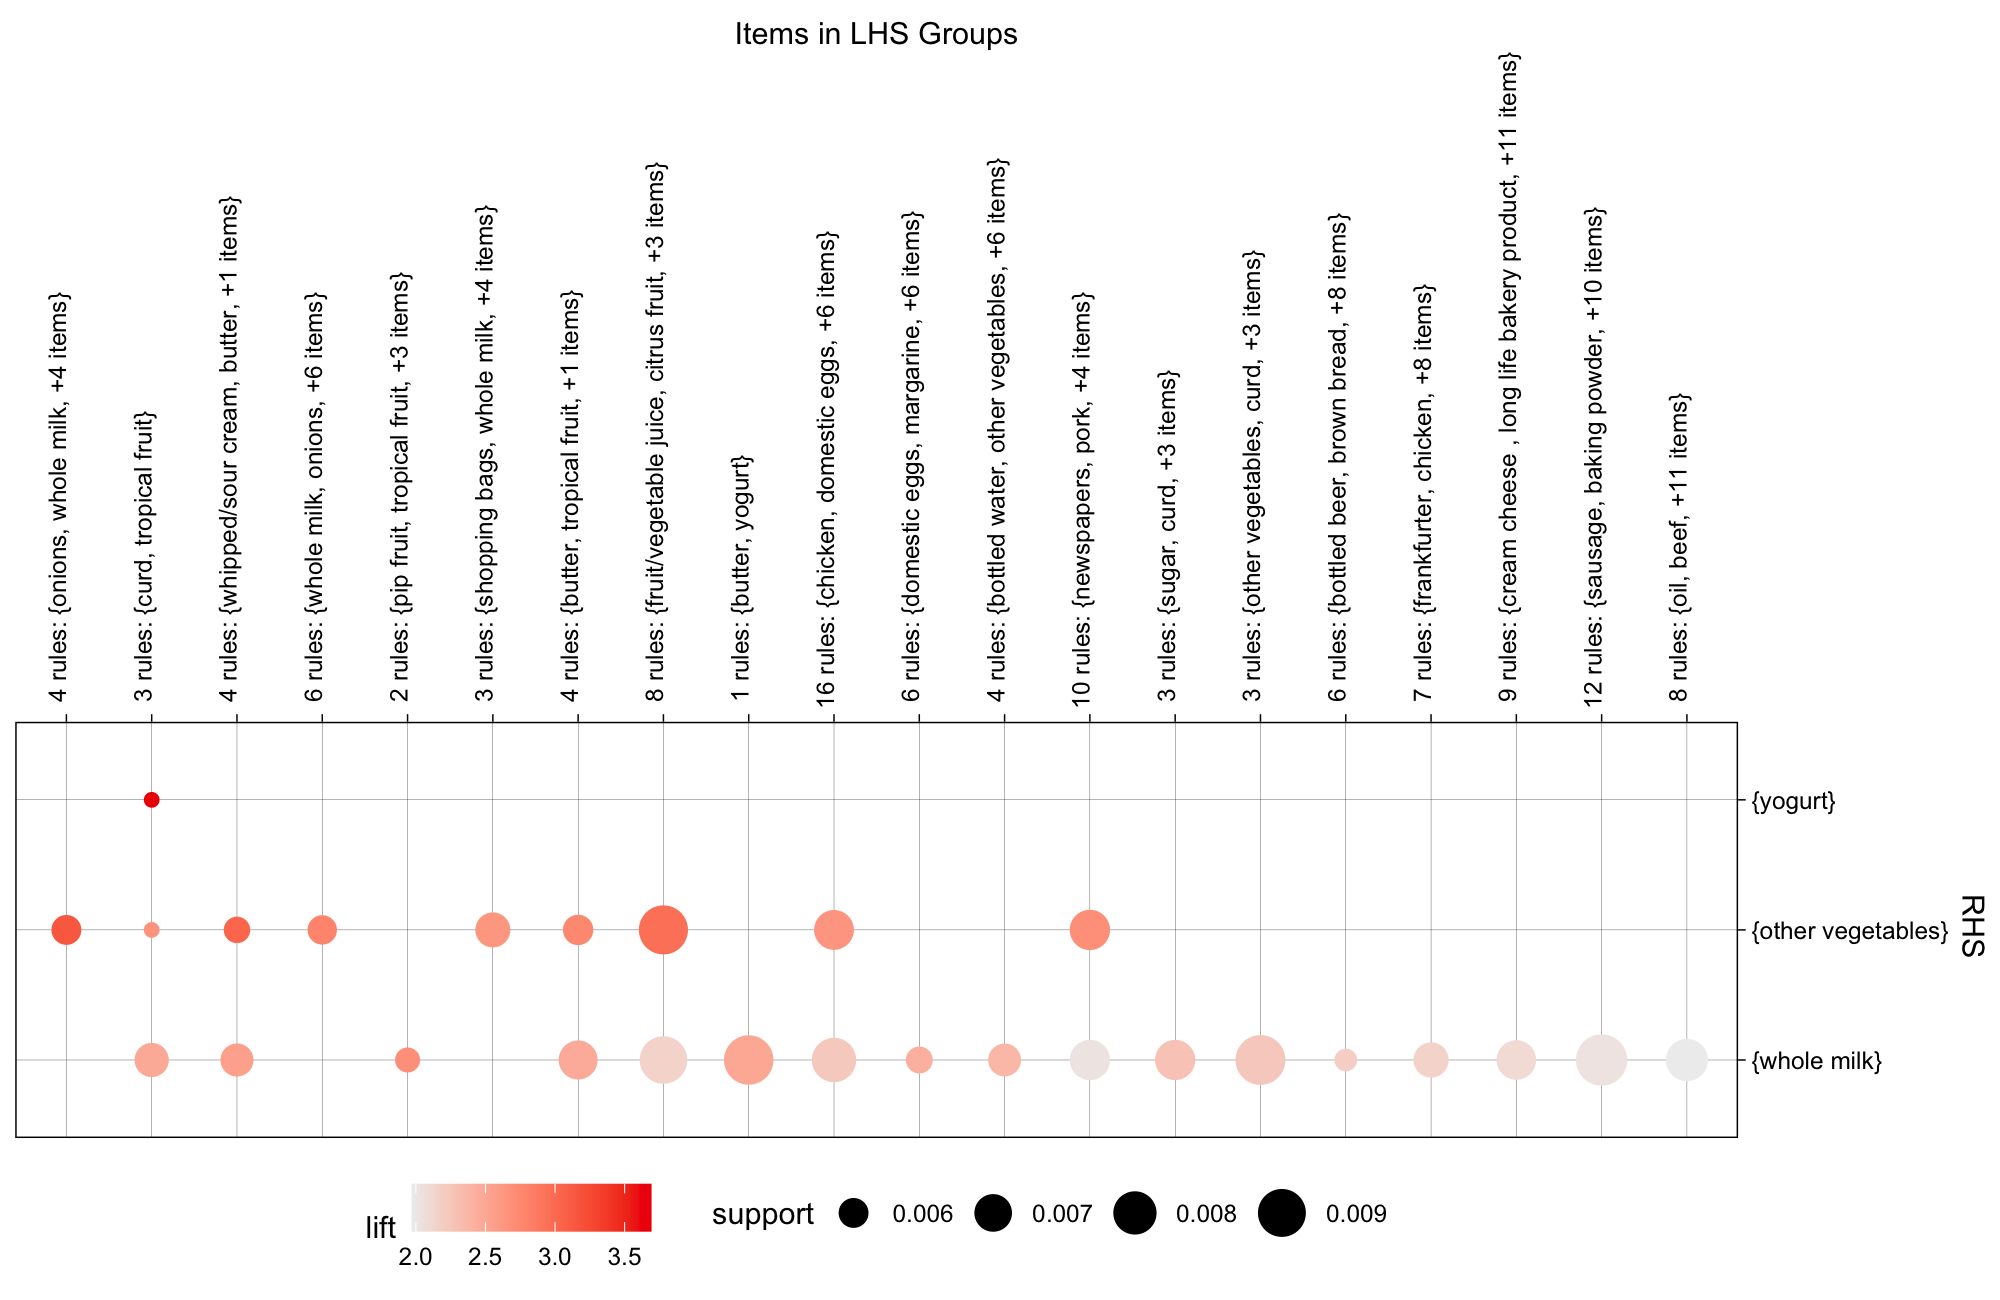
\includegraphics[width=\textwidth]{grouped_matrix.png}
  \caption{Matriz agrupada de las 119 reglas limpias: grupos de antecedentes (columnas)
  frente a consecuentes (filas).}
  \label{fig:grouped}
\end{figure}

\section{Retos}

\subsection{Reto 1: \emph{bottled beer} frente a \emph{soda}}

Para capturar patrones de nicho se bajaron los umbrales a \texttt{supp = 0.001} y
\texttt{conf = 0.15}, lo que produce 26\,820 reglas. De ellas, 523 contienen
\texttt{bottled beer} en el LHS y 1\,935 contienen \texttt{soda}. Las
Tablas~\ref{tab:beer} y~\ref{tab:soda} presentan las cinco de mayor \emph{lift} para cada
bebida.

\begin{table}[H]
  \centering
  \caption{Las 5 reglas de mayor \emph{lift} con \texttt{bottled beer} en el LHS}
  \label{tab:beer}
  \small
  \begin{tabular}{llrrrr}
    \toprule
    LHS & RHS & Soporte & Confianza & Lift & Conteo \\
    \midrule
    \{bottled beer, red/blush wine\} & liquor & 0.0019 & 0.396 & 35.72 & 19 \\
    \{bottled beer, liquor\} & red/blush wine & 0.0019 & 0.413 & 21.49 & 19 \\
    \{tropical fruit, whole milk, bottled beer\} & white bread & 0.0010 & 0.323 & 7.66 & 10 \\
    \{citrus fruit, bottled beer\} & oil & 0.0010 & 0.167 & 5.94 & 10 \\
    \{whole milk, domestic eggs, bottled beer\} & margarine & 0.0010 & 0.345 & 5.89 & 10 \\
    \bottomrule
  \end{tabular}
\end{table}

\begin{table}[H]
  \centering
  \caption{Las 5 reglas de mayor \emph{lift} con \texttt{soda} en el LHS}
  \label{tab:soda}
  \small
  \begin{tabular}{llrrrr}
    \toprule
    LHS & RHS & Soporte & Confianza & Lift & Conteo \\
    \midrule
    \{hamburger meat, soda\} & Instant food products & 0.0012 & 0.211 & 26.21 & 12 \\
    \{Instant food products, soda\} & hamburger meat & 0.0012 & 0.632 & 19.00 & 12 \\
    \{soda, popcorn\} & salty snack & 0.0012 & 0.632 & 16.70 & 12 \\
    \{whole milk, white bread, soda\} & processed cheese & 0.0010 & 0.250 & 15.08 & 10 \\
    \{ham, soda\} & processed cheese & 0.0010 & 0.204 & 12.31 & 10 \\
    \bottomrule
  \end{tabular}
\end{table}

El folclore de la tienda se confirma. Las reglas de \texttt{soda} están dominadas por comida
rápida y pasabocas: carne de hamburguesa, productos instantáneos, palomitas, snacks salados y
queso procesado. Las de \texttt{bottled beer} no contienen ningún pasabocas. Sus dos reglas
más fuertes vinculan la cerveza con licor y vino, un resultado esperable: quien compra un
tipo de alcohol suele comprar otro.

El ítem más sorprendente correlacionado positivamente con \texttt{bottled beer} es
\texttt{white bread} (\emph{lift} 7.66), seguido de \texttt{oil} y \texttt{margarine}: la
cerveza embotellada aparece en canastas de despensa cotidiana y no en canastas de fiesta.
Esta lectura debe tomarse con cautela, porque las reglas 3 a 5 se apoyan en solo 10 recibos
cada una, exactamente el mínimo que permite el umbral de soporte.

\subsection{Reto 2: correlaciones negativas (\emph{lift} $< 1$)}

Se ejecutó \texttt{apriori()} con \texttt{supp = 0.01}, \texttt{conf = 0.05} y
\texttt{minlen = 2}, y se obtuvieron 513 reglas. El filtro propuesto, \emph{lift} $< 0.75$,
devuelve cero reglas: el \emph{lift} mínimo de todo el conjunto es 0.79. Por ello se relajó
el filtro a \emph{lift} $< 1$, que conserva 20 reglas (Tabla~\ref{tab:neg}).

\begin{table}[H]
  \centering
  \caption{Las 6 reglas de menor \emph{lift}}
  \label{tab:neg}
  \begin{tabular}{llrrrr}
    \toprule
    LHS & RHS & Soporte & Confianza & Lift & Conteo \\
    \midrule
    \{rolls/buns\} & canned beer & 0.0113 & 0.061 & 0.790 & 111 \\
    \{canned beer\} & rolls/buns & 0.0113 & 0.145 & 0.790 & 111 \\
    \{citrus fruit\} & soda & 0.0128 & 0.155 & 0.888 & 126 \\
    \{soda\} & citrus fruit & 0.0128 & 0.073 & 0.888 & 126 \\
    \{soda\} & whole milk & 0.0401 & 0.230 & 0.899 & 394 \\
    \{whole milk\} & soda & 0.0401 & 0.157 & 0.899 & 394 \\
    \bottomrule
  \end{tabular}
\end{table}

El par de menor \emph{lift} es \texttt{rolls/buns} y \texttt{canned beer}. Aparece dos veces
con el mismo valor porque el \emph{lift} es simétrico. A partir de los soportes individuales
(1\,809 y 764 recibos) y del soporte conjunto (111 recibos de 9\,835), la
Ecuación~\ref{eq:medidas} da:
\begin{equation}
  \text{lift} = \frac{\text{supp}(A \cup B)}{\text{supp}(A)\,\text{supp}(B)}
  = \frac{0.01129}{0.18393 \times 0.07768} = \frac{0.01129}{0.01429} = 0.790,
\end{equation}
valor que coincide con el reportado por \texttt{apriori()}.

En lenguaje llano: si los dos productos fueran independientes, se esperaría encontrarlos
juntos en el 1.43\% de los recibos (unos 141), pero solo aparecen juntos en 111, cerca de un
21\% menos de lo esperado por azar. Una interpretación plausible es que corresponden a
misiones de compra distintas: la cerveza en lata se compra en viajes dedicados a bebidas,
mientras que los panes forman parte de la compra diaria de alimentos. Los datos muestran la
repulsión, no su causa, y con 0.79 se trata de una repulsión moderada.

El filtro original queda vacío por una razón estructural. Para existir como regla, un par
debe coincidir en al menos el 1\% de los recibos, y dos productos que realmente se evitan
rara vez coinciden tanto. Con \texttt{supp = 0.005} sí aparecen repulsiones fuertes, como
\{canned beer\} $\Rightarrow$ whole milk con \emph{lift} 0.45.

\subsection{Reto 3: el censo \emph{Adult}}

El dataset \emph{Adult} contiene 48\,842 registros y 115 ítems, donde cada ítem es un par
atributo--valor (por ejemplo, \texttt{education=Bachelors}). Se minaron reglas que predicen
ingresos altos fijando el RHS en \texttt{income=large}, con \texttt{supp = 0.02} y
\texttt{conf = 0.50}. Solo se generan 6 reglas, y tras eliminar las redundantes quedan 2
(Tabla~\ref{tab:adult}, Figura~\ref{fig:adult}).

\begin{table}[H]
  \centering
  \caption{Reglas no redundantes que predicen \texttt{income=large}}
  \label{tab:adult}
  \small
  \begin{tabular}{lrrrr}
    \toprule
    LHS & Soporte & Confianza & Lift & Conteo \\
    \midrule
    \{capital-gain=High, native-country=United-States\} & 0.0212 & 0.672 & 4.19 & 1\,035 \\
    \{capital-gain=High\} & 0.0232 & 0.670 & 4.18 & 1\,133 \\
    \bottomrule
  \end{tabular}
\end{table}

\begin{figure}[H]
  \centering
  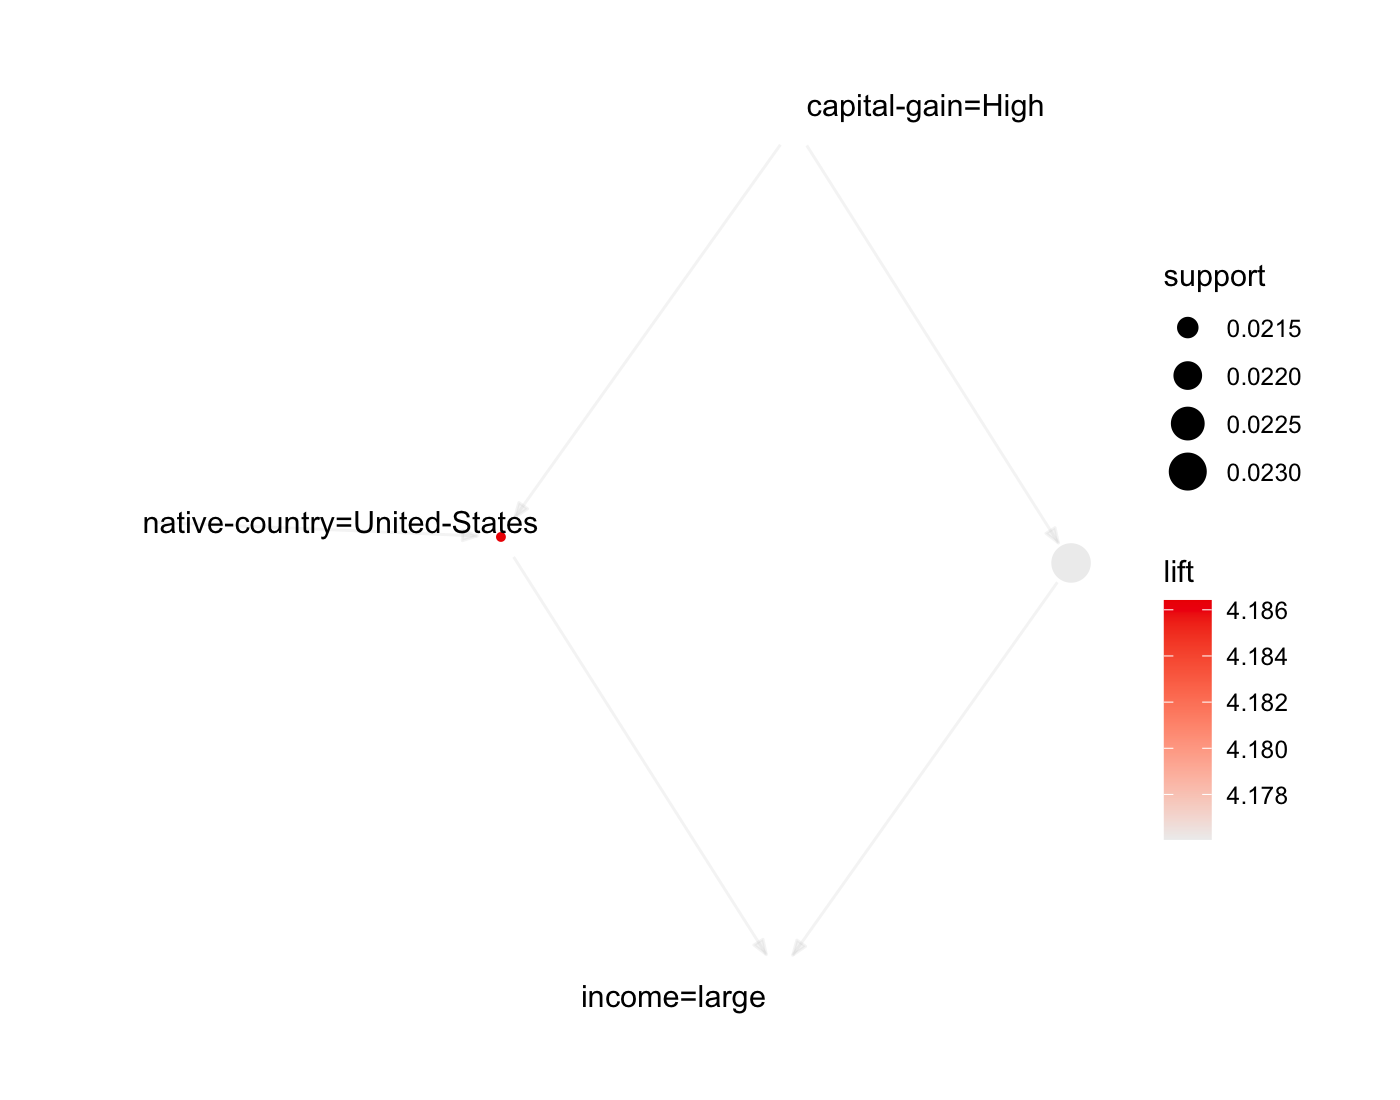
\includegraphics[width=0.7\textwidth]{adult_graph.png}
  \caption{Grafo de las reglas que predicen \texttt{income=large}. El círculo gris es la
  regla \{capital-gain=High\}; el punto rojo, la que añade \texttt{native-country=United-States}.}
  \label{fig:adult}
\end{figure}

El conjunto es tan pequeño porque \texttt{income=large} aparece solo en el 16.1\% de los
registros (en un tercio del dataset el ingreso no está registrado), de modo que una confianza
del 50\% es una barrera alta que únicamente supera la ganancia de capital. Las cuatro reglas
eliminadas añadían \texttt{capital-loss=None} o \texttt{race=White} sin mejorar la confianza.
La diferencia de color de la Figura~\ref{fig:adult} es engañosa: la escala de \emph{lift}
solo abarca de 4.176 a 4.186, por lo que ambas reglas tienen prácticamente la misma fuerza.

\textbf{Resumen.} El factor con mayor correlación positiva con un ingreso alto es la
ganancia de capital elevada: el 67\% de las personas con \texttt{capital-gain=High} gana un
ingreso alto, frente al 16\% de la población general, lo que equivale a un \emph{lift} de 4.2.
Con los umbrales del reto ningún factor demográfico o laboral supera por sí solo el 50\% de
confianza; al relajar la confianza a 0.40 (exploración adicional, 59 reglas no redundantes)
el siguiente grupo corresponde a personas casadas del sector privado con cargos
ejecutivos o con título de pregrado, con \emph{lift} cercano a 3. Ordenar por \emph{lift} es
más informativo que ordenar por soporte porque el soporte solo indica qué tan común es un
grupo, mientras que el \emph{lift} indica cuánto más probable que el promedio es que ese grupo
tenga un ingreso alto.

\section{Conclusiones}

\begin{enumerate}
  \item El dataset \emph{Groceries} es muy disperso (densidad 0.026, mediana de 3 ítems por
        recibo) y está dominado por unos pocos productos: \texttt{whole milk} aparece en uno
        de cada cuatro recibos.
  \item El soporte y la confianza favorecen a los ítems populares. Los diez conjuntos más
        frecuentes de Eclat y las cinco reglas de mayor confianza de Apriori giran alrededor
        de \texttt{whole milk}, mientras que el \emph{lift} destaca asociaciones específicas
        como \{tropical fruit, curd\} $\Rightarrow$ yogurt (3.69).
  \item Los umbrales determinan lo que se puede descubrir. Una confianza mínima del 50\%
        limita los consecuentes a tres ítems, deja sin respuesta la pregunta sobre
        \texttt{berries} y filtra por completo las correlaciones negativas.
  \item Las frutas, verduras y lácteos frescos forman el grupo de asociaciones más sólido:
        \texttt{other vegetables} es el destino de 14 de las 15 reglas de mayor \emph{lift}.
  \item Los patrones de consumo de \texttt{soda} y \texttt{bottled beer} son distintos: la
        gaseosa se asocia con comida rápida y pasabocas, y la cerveza embotellada con otras
        bebidas alcohólicas y productos de despensa.
  \item Las correlaciones negativas encontradas son moderadas. El par de menor \emph{lift}
        con soporte de 1\% es \texttt{rolls/buns} y \texttt{canned beer} (0.79), valor
        verificado manualmente a partir de los soportes individuales.
  \item La minería de reglas se aplica a cualquier dataset categórico: en \emph{Adult}, la
        ganancia de capital elevada multiplica por 4.2 la probabilidad de un ingreso alto.
  \item Limitaciones: las reglas con soporte cercano al umbral se apoyan en muy pocos recibos
        (10 en el Reto 1), las reglas describen coocurrencia y no causalidad, y tres filtros
        del laboratorio devolvieron resultados vacíos o casi vacíos con los parámetros
        indicados, por lo que se reportan junto a exploraciones adicionales claramente
        señaladas.
\end{enumerate}

\appendix
\section{Código fuente}

El código completo del laboratorio (carga de datos, exploración, Eclat, Apriori, poda,
visualizaciones y los tres retos) se encuentra en el script \texttt{main.R}. Se ejecutó con
R 4.6.2, \texttt{arules} 1.7.15 y \texttt{arulesViz} 1.5.4 \cite{arulesviz2017}. El script
genera el grafo de las 15 reglas de mayor \emph{lift} como un widget interactivo
(\texttt{engine = "htmlwidget"}); para este documento se exportó la versión estática
equivalente de la misma llamada.

\begin{thebibliography}{9}
  \bibitem{arules2005} Hahsler, M., Grün, B., \& Hornik, K. (2005).
    arules -- A computational environment for mining association rules and frequent item sets.
    \emph{Journal of Statistical Software}, 14(15), 1--25.
  \bibitem{groceries2006} Hahsler, M., Hornik, K., \& Reutterer, T. (2006).
    Implications of probabilistic data modeling for mining association rules.
    En \emph{From Data and Information Analysis to Knowledge Engineering} (pp. 598--605). Springer.
  \bibitem{agrawal1994} Agrawal, R., \& Srikant, R. (1994).
    Fast algorithms for mining association rules.
    \emph{Proceedings of the 20th International Conference on Very Large Data Bases (VLDB)}, 487--499.
  \bibitem{zaki2000} Zaki, M. J. (2000).
    Scalable algorithms for association mining.
    \emph{IEEE Transactions on Knowledge and Data Engineering}, 12(3), 372--390.
  \bibitem{arulesviz2017} Hahsler, M. (2017).
    arulesViz: Interactive visualization of association rules with R.
    \emph{The R Journal}, 9(2), 163--175.
  \bibitem{adult1996} Becker, B., \& Kohavi, R. (1996).
    Adult. \emph{UCI Machine Learning Repository}.
    \url{https://archive.ics.uci.edu/dataset/2/adult}
\end{thebibliography}

\end{document}
